%%% Template originaly created by Karol Kozioł (mail@karol-koziol.net) and modified for ShareLaTeX use

\documentclass[a4paper,11pt]{article}

\usepackage[T1]{fontenc}
\usepackage[utf8]{inputenc}
\usepackage{graphicx}
\usepackage{xcolor}
\usepackage{pgf}
\usepackage{tikz}
\usetikzlibrary{arrows,automata}
\usepackage{tgtermes}

\usepackage[
pdftitle={ML assignement}, 
pdfauthor={Salma El Alaoui Talibi},
colorlinks=true,linkcolor=blue,urlcolor=blue,citecolor=blue,bookmarks=true,
bookmarksopenlevel=2]{hyperref}
\usepackage{amsmath,amssymb,amsthm,textcomp}
\usepackage{enumerate}
\usepackage{multicol}
\usepackage{tikz}
\usepackage{subcaption}
\usepackage{geometry}
\geometry{total={210mm,297mm},
left=25mm,right=25mm,%
bindingoffset=0mm, top=20mm,bottom=20mm}


\linespread{1.3}

\newcommand{\linia}{\rule{\linewidth}{0.5pt}}

% custom theorems if needed
\newtheoremstyle{mytheor}
    {1ex}{1ex}{\normalfont}{0pt}{\scshape}{.}{1ex}
    {{\thmname{#1 }}{\thmnumber{#2}}{\thmnote{ (#3)}}}

\theoremstyle{mytheor}
\newtheorem{defi}{Definition}

% my own titles
\makeatletter
\renewcommand{\maketitle}{
\begin{center}
\vspace{2ex}
{\huge \textsc{\@title}}
\vspace{1ex}
\\
\linia\\
\@author \hfill \@date
\vspace{4ex}
\end{center}
}
\makeatother
%%%

% custom footers and headers
\usepackage{fancyhdr,lastpage}
\pagestyle{fancy}
\lhead{}
\chead{}
\rhead{}
\lfoot{Assignment \textnumero{} 1 -- Salma El Alaoui Talibi}
\cfoot{}
\rfoot{Page \thepage\ /\ \pageref*{LastPage}}
\renewcommand{\headrulewidth}{0pt}
\renewcommand{\footrulewidth}{0pt}
%

%%%----------%%%----------%%%----------%%%----------%%%

\begin{document}

\title{DD$2434$ Machine Learning, Advanced Course\\ Assignment 1 }

\author{Salma El Alaoui Talibi (931007-T148)}

\date{\today}

\maketitle

\section{The prior}

\subsection{Theory}

\fbox{
  \parbox{\textwidth}{
\textbf{Question 1: }\textit{Why is choosing a Gaussian likelihood a sensible thing to do? What does it mean that we have chosen a spherical covariance matrix for the likelihood?}
  }
}
\smallskip
\\Since we have no previous knowledge about the uncertainty in the observations, we can assume that the source of this uncertainty is a large number of measurement errors that are independent and identically distributed. According to the Central Limit Therorem, the noise resulting from this sum of errors will be normally distributed. Since the likelihood is for a given $f$ and $x_i$, it only depends on the noise, and therefore it is sensible to assume that the likelihood is Gaussian.\\
A spherical covariance matrix for the likelihood means that the components $y^{j}_j$ of the vector $y_i$ do not covary with each other conditionally given $f$ and $x_{i}$, which means they are uncorrelated. 
\begin{equation*}
\forall i \leq N , \; \forall j,k\leq D \;j \neq k  \quad cov(y^j_{i}, y^k_{i} | f, x_i ) = 0
\end{equation*} 
The variance of all the components $y^{j}_j$ of the vector $y_i$ conditionally given $f$ and $x_{i}$ is constant and equal.
\begin{equation*}
\forall i \leq N \quad var(y^j_{i}| f, x_i ) = \sigma^2
\end{equation*} 
\smallskip
\fbox{
  \parbox{\textwidth}{
\textbf{Question 2: }\textit{If we do not assume that the data points are independent how would the likelihood
look then?}
  }
}
\smallskip
\\By applying the product rule, we obtain:
\begin{equation*}
p \left({Y| f, X} \right) = p \left ({y_N | f, X} \right) \prod\limits_{i=1}^{N - 1} p\left ({y_i|y_{i+1},\ldots,y_{N-1},y_N,f,X} \right)
\end{equation*}
\subsubsection{Linear Regression}
\fbox{
  \parbox{\textwidth}{
\textbf{Question 3: }\textit{What is the specific form of the likelihood above, complete the right-hand side of the expression.}
  }
}
\smallskip
\\We assume our observations are corrupted by additive noise, that is normally distributed.Therefore, the likelihood has the following form:
\begin{equation*}
p \left({Y|W, X} \right) = \prod\limits_{i=1}^{N} p \left(y_{i}|W,x_{i}\right) \quad \text{where} \quad p \left(y_{i}|W,x_{i}\right) = \mathcal{N}(W x_i, \sigma^2I) 
\end{equation*}
\smallskip
\fbox{
  \parbox{\textwidth}{
\textbf{Question 4: }\textit{Explain the concept of conjugate distributions. Why is this a motivated choice?}
  }
}
\smallskip
\\The likelihood function is a Gaussian with a known variance, so a Gaussian prior would be a conjugate to the likelihood function. This way, the posterior will have the same functional form as the prior, ie a Gaussian, and we will only need to estimate its parameters.
\smallskip
\\\\\fbox{
  \parbox{\textwidth}{
\textbf{Question 5: }\textit{The prior in Eq.8 is a spherical Gaussian. This means that the "preference" is
encoded in terms of a L2 distance in the in the space of the parameters. With this view, how
would the preference change if the preference was rather encoded using a L1 norm? Compare
and discuss the different type of solutions these two priors would encode.}
  }
}
\smallskip
\\If the preference was encoded using a L1 norm, that would mean that we would choose a Laplace distribution to model the prior, ie $ W \sim \frac{\sqrt\lambda}{2} e^{-\sqrt\lambda|W|}$.\\
the Laplace distribution is peaked at the mean while the Gaussian distribution is smooth around the mean, therefore The laplacian prior assigns more weight to regions near
the mean than the normal prior. If we have no prior knowledge about this mean and take it to be 0 by symmetry, it expresses the prior belief that the distribution of feature relevances with relation to the target is strongly peaked around zero.
If one of the components of W  happens to be irrelevant, a Gaussian prior will not set it exactly to zero, but will prune it to some small value. On the other hand, under a Laplacian prior, some of the components of W may be exactly zero.
\smallskip
\\\\\fbox{
  \parbox{\textwidth}{
\textbf{Question 6: }\textit{Derive the posterior over the parameters. I recommend that you do these calculations by hand as it is very good practice. However, in order to pass the assignment you only
need to outline the calculation and highlight the important steps.
Why does it have the form that it does?\\
What is the effect of the constant Z, are we interested in this?}
  }
}
\smallskip
\\The likelihood of the data has the following form:
\begin{equation*}
p \left({Y|W, X} \right) = \prod\limits_{i=1}^{N} p \left(y_{i}|W,x_{i}\right) \quad \text{where} \quad p \left(y_{i}|W,x_{i}\right) = \mathcal{N}(W x_i, \sigma^2I) 
\end{equation*}
Since the product of Gaussians is a Gaussian, and the covariance matrix for the likelihood of each point $y_i$ is spherical, we can write the likelihood as :
\begin{equation*}
p \left({Y|W, X} \right) = \mathcal{N}(WX, \sigma^2I)
\end{equation*}
We choose a Gaussian prior with a zero mean over the parameter:
\begin{equation*}
p \left(W\right) = \mathcal{N}(0, \Sigma)
\end{equation*}
The pdf of a general normal has the following form:
\begin{equation*}
\mathcal{N}(\mu, \Sigma) \propto e^{\frac{-1}{2}(x-\mu)^T\Sigma^{-1}(x-\mu)}
\end{equation*}
According to Bayes rule, we write the posterior as: 
\begin{equation*}
p(W|Y,X) \propto p(Y|W,X) p(W)
    \propto e^{\frac{-1}{2\sigma^2} (y-XW)^T(y-XW)}\; e^{\frac{-1}{2}W^T\Sigma^{-1}W}
\end{equation*}
Gaussians are self-conjugate, so a Gaussian prior and a Gaussian likelihood give a Gaussian posterior, ie $\mathcal{N}(\mu, S)$. We rewrite the exponent as:
\begin{equation*}
\frac{-1}{2\sigma^2} (y-XW)^T(y-XW)\frac{-1}{2}W^T\Sigma^{-1}W
=\frac{-1}{2\sigma^2} Y^TY + \frac{1}{2\sigma^2}Y^T(XW)-\frac{1}{2\sigma^2}(XW)^T(XW)-\frac{1}{2}W\Sigma^{-1}W
\end{equation*}
The first term (A) is the constant term of the normal, the second term (B) is the mixed term and the two last terms (C) correspond to the terms with a quadratic in parameters.\\
By rewriting (C), we obtain:
\begin{equation*}
C = \frac{-1}{2}W^T(\frac{1}{\sigma^2}X^TX + \sigma^{-1})W
\end{equation*}
We can therefore identify the inverse covariance matrix of the posterior as:
\begin{equation*}
S^{-1} = \frac{1}{\sigma^2}X^TX + \Sigma^{-1}
\end{equation*}
By rewriting the term (B) it we obtain:
\begin{equation*}
B = \frac{1}{2\sigma^2} W^TX^TY
\end{equation*}
Since the mean appears in the mixed term, we can write using the expression of the covariance matrix that we previously found:
\begin{equation*}
\frac{1}{2\sigma^2} W^TX^TY = W^T(\frac{1}{\sigma^2}X^TX + \sigma^{-1})\mu
\end{equation*}
After solving for $\mu$, we obtain:
\begin{equation*}
\mu = \frac{1}{\sigma^2}(\frac{1}{\sigma^2} X^TX + \Sigma^{-1})^{-1}X^TY
\end{equation*}
The constant Z is a normalising constant so that the posterior represents a true probability distribution, ie $p(W|Y,X) =\frac{1}{Z}p(Y|W,X) p(W) \leq 1$. Z represents the evidence, which we will use for model selection.
\subsubsection{Non-parametric Regression}

\fbox{
  \parbox{\textwidth}{
\textbf{Question 7: }\textit{What is a non-parametric model and what is the difference between non-parametrics
and parametrics? In specific discuss these two aspects of non-parametrics: representability and interpretability?}
  }
}
\smallskip
\\ In a non-parametric model, we do not give the function between the two variates a predefined specific form, but instead define a prior probability distribution over functions directly.\\
While the validity of parametric
models relies on the correctness of the specified model, non-parametric models assumes no specific form of the function, and adapt
to the underlying function using the empirical
data. Therefore non-parametric models provide a better representability and goodness of fit to the data.\\
However, parametric model have directly interpretable parameters, while non-parametric yield relationship that are difficult to describe, especially if the we map the features to spaces with high or infinite dimensionality. Therefore parametric models give better interpretability.
\smallskip
\\\\
\fbox{
  \parbox{\textwidth}{
\textbf{Question 8: }\textit{Explain what this prior does? Why is it a sensible choice? Use images to show your reasoning. Clue: use the marginal distribution to explain the prior}
  }
}
\smallskip
\\ The Gaussian process allows us to define a prior probability distribution over functions directly. We know 2 points about the mapping $f$ between $Y$ and $X$: 
\begin{enumerate}
\item it's a function, ie: $ \forall x_i \in \mathbb{R}^q,  \; \exists ! y_i \in \mathbb{R}^D\;/ \; f(x_i) = y_i $
\item $ f(x_i) \in \mathbb{R}^D$, which means that we can map an input to any value in our output space.
\end{enumerate}
If we choose a Gaussian process, ie $p(f|X,\theta) = \mathcal{N}(0, k(X,X)) $, then according to the definition of a Gaussian process, the marginal distribution $p(f)$ is Gaussian, which has the following characteristics: 
\begin{itemize}
\item A Gaussian is uni-modal, which addresses point 1.
\item the pdf of a Gaussian is such that $f(x|\mu, \sigma) > 0$, which addresses point 2.
\end{itemize}
All instantiations of the function are jointly Gaussian, and covariance allows us to express that for points $x_i$ and $x_j$ that are similar, the corresponding values $f_i$ and $f_j$ will be more strongly correlated than for dissimilar points. The parameter $\theta$ defines this similarity, which allows us to control the smoothness of the function, for example.
\smallskip
\\\\
\fbox{
  \parbox{\textwidth}{
\textbf{Question 9: }\textit{Formulate the joint likelihood of the full model that you have defined above, $p(Y, X, f, \theta)$. Draw the graphical model to clearly show the assumptions that you have made.}
  }
}
\smallskip
\\ We know that X and $\theta$ are independent. We also know that Y is conditionally independent of X and $\theta$ given f (Y depends on X, but all the information in X relevant to determine Y is captured by f and $\theta$).\\
This gives us the following Bayesian network:\\
\begin{center}
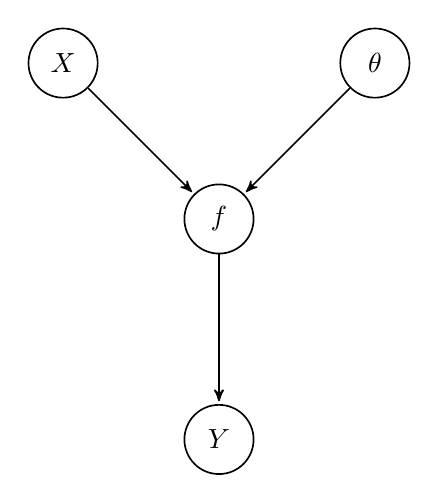
\begin{tikzpicture}[->,>=stealth',shorten >=1pt,auto,node distance=2.8cm,
                    semithick]
  

  \node[state] (Y)                    {$Y$};
  \node[state]         (f) [above of=Y] {$f$};
  \node[state]         (O) [above right of=f] {$\theta$};
  \node[state]         (X) [above left of=f] {$X$};

  \path (O) edge              node {} (f)
        (X) edge              node {} (f)
        (f) edge              node {} (Y);
\end{tikzpicture}
\end{center}
The joint likelihood for this model is therefore:
\begin{equation*}
p(Y,X,f,\theta) = p(Y|f) p(f|X,\theta) p(X) p(\theta)
\end{equation*}
\smallskip
\\
\fbox{
  \parbox{\textwidth}{
\textbf{Question 10: }\textit{Explain the marginalisation in Eq.12. Explain how this connects the prior and the data? How does the uncertainty filter through this? What does it imply that $\theta$ is left on the left-hand side of the expression after marginalisation?}
  }
}
\smallskip
\begin{equation*}
 p(Y|X,\theta) = \int p(Y|f)p(f|X,\theta)df
\end{equation*}

\begin{itemize}
\item We average the likelihood of the data points over all possible functions given by the prior over function realisations.
\item We merge the uncertainty in the observations given by $p(Y|f)$ with the uncertainty in the relationship between X and Y given by $p(f|X,\theta)$.
\item Since we average over all functions of the Gaussian process, $\theta$ is constant in this integral, therefore the result is a function of $\theta$.
\end{itemize}

\subsection{Practical}
\subsubsection{Linear Regression}
\fbox{
  \parbox{\textwidth}{
\textbf{Question 11: }\textit{Describe the plots, and the behavior when adding more data? Is this a desirable behavior?}
  }
}
\smallskip

\begin{figure}[h]
\centering
\includegraphics[scale =0.5]{prior} 
\caption{Prior Distribution over W}
\end{figure}

\begin{figure}[h]
\begin{subfigure}{0.5\textwidth}
\includegraphics[width=\linewidth, height=6cm]{posterior-1point} 
\caption{Posterior Distribution over W}
\end{subfigure}
\begin{subfigure}{0.5\textwidth}
\includegraphics[width=\linewidth, height=6cm]{samples-1point}
\caption{Samples from the posterior}
\end{subfigure}
\caption{After 1 observation}
\label{fig:one}
\end{figure}

\begin{figure}[h]
\begin{subfigure}{0.5\textwidth}
\includegraphics[width=\linewidth, height=6cm]{posterior-2points} 
\caption{Posterior Distribution over W}
\end{subfigure}
\begin{subfigure}{0.5\textwidth}
\includegraphics[width=\linewidth, height=6cm]{samples-2points}
\caption{Samples from the posterior}
\end{subfigure}
\caption{After 2 observations}
\label{fig:two}
\end{figure}

\begin{figure}[h]
\begin{subfigure}{0.5\textwidth}
\includegraphics[width=\linewidth, height=6cm]{posterior-final} 
\caption{Posterior Distribution over W}
\end{subfigure}
\begin{subfigure}{0.5\textwidth}
\includegraphics[width=\linewidth, height=6cm]{samples-final}
\caption{Samples from the posterior}
\end{subfigure}
\caption{After 25 observations}
\label{fig:final}
\end{figure}

After observing a single data point (figure \ref{fig:one}), the posterior becomes constrained by the corresponding likelihood. When we sample from the posterior and draw it in the data space, there are many possible solutions with different slopes/intercepts, which makes sense since we cannot infer two parameters from one observation. After we see two data points (figure \ref{fig:two}), the posterior becomes narrower, and the samples from the posterior have similar slopes and intercepts than before. After 25 observations (figure \ref{fig:final}), we can see that the posterior is centered on the true value, $w0 = -1.3$ and $w1 = 0.5$.
Since the data was generated from this model, this is the desirable behavior because the estimate converges to the true value.

\subsubsection{Non-parametric Regression}
\fbox{
  \parbox{\textwidth}{
\textbf{Question 12: }\textit{Create a $\mathcal{GP}$-prior with a squared exponential co-variance function, sample from this prior and visualise the samles
and show samples using different length-scale for the squared exponential.\\
Explain the behavior of altering the length-scale of the covariance function.}
  }
}
\smallskip
\\
\begin{figure}[h]
\begin{subfigure}{0.5\textwidth}
\includegraphics[width=\linewidth, height=6cm]{lverysmall}
\caption{Length-scale = 0.02}
\label{fig:un}
\end{subfigure}
\begin{subfigure}{0.5\textwidth}
\includegraphics[width=\linewidth, height=6cm]{lsmall}
\caption{Length-scale = 0.2}
\end{subfigure}
\begin{subfigure}{0.5\textwidth}
\includegraphics[width=\linewidth, height=6cm]{lmedium}
\caption{Length-scale = 2}
\end{subfigure}
\begin{subfigure}{0.5\textwidth}
\includegraphics[width=\linewidth, height=6cm]{lbig}
\caption{Length-scale = 20}
\label{fig:cor}
\end{subfigure}
\caption{Samples from the $\mathcal{GP}$ with different length-scales}
\label{fig:lengthscale}
\end{figure}
As we can observe in figure \ref{fig:lengthscale}, the larger the length scale the smoother the samples become.
The squared exponential covariance of a $\mathcal{GP}$ has the following form : $k(x_i, x_j) = \sigma^2_f e{-\frac{(x_i-x_j)^T(x_i-x_j)}{l^2}}$.\\For a constant squared euclidean distance between two points $x_i$ and $x_j$, the larger $l$, the larger $k(x_i, x_j)$ is, which means that the instantiations $f_i$ and $f_j$ will be more strongly correlated. For a very small value of the length-scale ( $l^2 \ll (x_i-x_j)^T(x_i-x_j)$ ), we can see that that the instantiations are uncorrelated even for very points that are very close (figure \ref{fig:un}). For a very large value, $l^2 \gg (x_i-x_j)^T(x_i-x_j)$, and all the points are equally strongly correlated (figure \ref{fig:cor}).
\smallskip
\\\\
\fbox{
  \parbox{\textwidth}{
\textbf{Question 13: }\textit{"The posterior and the prior are the same object if we do not have any observed data."\\ Explain the statement, why is this?}
  }
}
\smallskip
\\The predictive posterior is given by:
\begin{equation*}
    \begin{bmatrix}
     f \\
      f_* \\
     \end{bmatrix}
     \sim
     \mathcal{N} 
     \Bigg( 
     \begin{bmatrix}
     0 \\
     0 \\
     \end{bmatrix},
     \begin{bmatrix}
     k(X,X) & k(X,x_*) \\
     k(x_*, X) & k(x_*, x_*)\\
     \end{bmatrix}
     \Bigg)
\end{equation*}
If we do not have any observed data, the predictive posterior becomes:
\begin{equation*}
      f_* \sim \mathcal{N} (0 , k(x_*,x_*))
\end{equation*}
which is a sample from the $\mathcal{GP}$ prior.
\\\\
\fbox{
  \parbox{\textwidth}{
\textbf{Question 14: }\textit{
\begin{enumerate}
\item Compute the predictive posterior distribution of the model
\item Sample from this posterior with points both close to the data and far away from the observed data.
\item Plot the data, the predictive mean and the predictive variance of the posterior from the
data.
\end{enumerate}
Explain the behavior of the samples and compare the samples of the posterior with the ones from the prior. Is this behavior desirable? What would happen if you would add a diagonal co-variance matrix to the squared exponential?}
  }
}


\smallskip
\begin{figure}[h]
\centering
\includegraphics[scale = 0.6]{posamples}
\caption{Samples from the posterior over $[-2\pi, 2\pi]$, length-scale = 2}
\end{figure}

\begin{figure}[h]
\begin{subfigure}{0.5\textwidth}
\includegraphics[width=\linewidth, height=6cm]{sin} 
\caption{$\epsilon \sim \mathcal{N}(0,0.5)$}
\end{subfigure}
\begin{subfigure}{0.5\textwidth}
\includegraphics[width=\linewidth, height=6cm]{sinless}
\caption{$\epsilon \sim \mathcal{N}(0,0.05)$}
\end{subfigure}
\caption{Gaussian process regression over $[-2\pi, 2\pi]$, length-scale = 2}
\label{fig:gaussreg}
\end{figure}
\hfill \\
We apply non-parametric regression using a Gaussian process prior with an exponential kernel, to a data-set of 7 observations $yi$ such as $yi = sin(x_i) + \epsilon$, where $\epsilon$ is independent Gaussian noise and $x_i \in [-\pi,...,\pi]$. \\
In figure \ref{fig:gaussreg}, the green curve shows the the function $sin$ and the red points show the observations. The blue curve shows the the mean of the Gaussian process predictive distribution, and the shaded region corresponds to plus and minus \textbf{2} standard deviations. We observe how the uncertainty increases in the regions that are far from the data points. To the left and to the right, the predictive mean converges towards 0, the mean of the prior, and the standard deviation converges towards 1 ($ 2 \sigma = 2$ in figure \ref{fig:gaussreg}), which is the value of the parameter $\sigma_f$ used in the covariance function of the prior.
\begin{figure}[h]
\centering
\includegraphics[scale = 0.6]{diagonal}
\caption{Gaussian process regression with $p(f|X,\theta) \sim k(X*,X)+\sigma^2I$}
\label{diagonal}
\end{figure}
\\After adding a diagonal covariance matrix to the squared exponential in figure \ref{diagonal}, we observe that the conditional distribution doesn't pass exactly through the data points as it did in figure \ref{fig:gaussreg}. It is equivalent to adding independent Gaussian noise to each of the 
values of $y_n$ obtained by
evaluating the function at input
values $x_n$ with $p(f|X,\theta) \sim k(X*,X)$, a squared exponential covariance function.

\section{The Posterior $p(X|Y)$}

\subsection{Theory}

\fbox{
  \parbox{\textwidth}{
\textbf{Question 15: }\textit{Elaborate on this, why can one view a prior as encoding a preference?}
  }
}
\smallskip
\\Since there is a simple relationship between $W$ and $X$ in the linear model, specifying a prior over $X$ allows us to encode our preference of the form or the properties that the variable $X$ should have, and that automatically constraints the variable $W$.
\\\\
\smallskip
\fbox{
  \parbox{\textwidth}{
\textbf{Question 16: }\textit{What type of "preference" does this prior encode?}
  }
}
\smallskip
\\The prior $p(x) = \mathcal{N}(0,I)$ encodes our preference for latent variables x with independent dimensions: 
\begin{equation*}
\forall i \leq N , \; \forall j,k\leq D \;j \neq k  \quad cov(x_i^j, x^k_{i} | f, x_i ) = 0
\end{equation*}
\smallskip
\\Since there is a simple relationship between $W$ and $X$ in the linear model, specifying a prior over $X$ allows us to encode our preference of the form or the properties that the variable $X$ should have, and that automatically constraints the variable $W$.
\\\\
\smallskip
\fbox{
  \parbox{\textwidth}{
\textbf{Question 17: }\textit{Perform the marginalisation in Eq. 23 and write down the expression. As pre-
viously, I do recommend that you do this by hand but to pass the assignment you only need to
outline the calculations and show the approach that you would take?}
  }
}
\smallskip
\\for a single data $y_i \in \mathbb{R}^D$, we assume a linear and a non-parametric Gaussian process, hence:
\begin{equation*}
y_i = W x_i + \epsilon \quad \text{where}\quad \epsilon \sim \mathcal{N}(0, \sigma^2I)  
\end{equation*}
The likelihood can be written as:
\begin{equation*}
p(y_i|x_i, W) = \mathcal{N}(y_i|W x_i, \sigma^2 I)
\end{equation*}
We integrate over the latent variables to get the marginal likelihood:
\begin{equation*}
p(y_i|W) = \int p(y_i|x_i, W)p(x_i)dx_i
\end{equation*}
where $p(x_i) = \mathcal{N}(0,I)$ is the prior over the latent variables.\\
The product of 2 Gaussians is a Gaussian, the marginal distribution of the data is also Gaussian. We can derive it by completing the square in the exponent, or just by evaluating the mean and the covariance given that it is a Gaussian:
\begin{equation*}
\begin{split}
\mathbb{E}[y_i|W] &= \mathbb{E}[W x_i +\epsilon]\\
                &= W \mathbb{E}[x_i] + \mathbb{E}[\epsilon]\\
                &=0
\end{split}
\end{equation*}
\begin{equation*}
\begin{split}
cov[y_i,y_i|W] &= \mathbb{E}[(y_i -\mathbb{E}[y_i])(y_i -\mathbb{E}[y_i])^T]\\
&= \mathbb{E}[(W x_i +\epsilon)(W x_i +\epsilon)^T]\\
& = \mathbb{E}[W x_i x_i^T W^T] + \mathbb{E}[\epsilon \epsilon^T]\\
&= WW^T + \sigma^2I
\end{split}
\end{equation*}
The marginal distribution for each data point is:
\begin{equation*}
p(y_i|W) = \mathcal{N}(y_i| 0 , WW^T + \sigma^2I) 
\end{equation*}
The marginal distribution for the full data set is: 
\begin{equation*}
p(Y|W) = \prod\limits_{i=1}^{N} p(y_i|W)
\end{equation*}

\subsubsection{Learning}
\fbox{
  \parbox{\textwidth}{
\textbf{Question 18: }\textit{Compare the three estimation procedures above. \begin{itemize}
\item How are they different?
\item How are MAP and ML different when we observe more data?
\item Why is the two last expressions of Eq. 25 equal?
\end{itemize}
}}
}
\smallskip
\begin{itemize}
\item The MAP estimate is the mode of the posterior. Maximum likelihood is equivalent to MAP with a
uniform prior. If we write the equations in log space:
\begin{itemize}
\item Maximizing likelihoood is equivalent equivalent to minimizing sum squared error, ie minimizing :
\begin{equation*}
l(w) = -\frac{1}{2\sigma^2}\sum\limits_{i = 1}^{N}(y_i-W^Tx_i^2) + const
\end{equation*}
\item MAP is equivalent to minimizing:
\begin{equation*}
l(w) = -\frac{1}{2\sigma^2}\sum\limits_{i = 1}^{N}(y_i-W^Tx_i)^2 -\sum w_i^2 + const
\end{equation*}
\end{itemize}
MAP is more expensive than ML computationally.
\item When we observe more data, the data will dominate the posterior distribution, as it will overwhelm the prior, and the MAP estimate will coverge towards the MLE estimate.
\item According to Bayes' rule:
\begin{equation*}
p(W|Y,X) = \frac{p(Y|W,X)p(W)}{p(Y|X)} = \frac{p(Y|X,W)p(W)}{\int p(Y|X,W)pWdW}
\end{equation*}
Since p(Y|X) does not depend on W:
\begin{equation*}
argmax_W \;\frac{p(Y|X,W)p(W)}{\int p(Y|X,W)pWdW} = argamx_W \; p(Y|X,W)p(W)
\end{equation*}
\end{itemize}
\smallskip
\fbox{
  \parbox{\textwidth}{
\textbf{Question 19: }\textit{
\begin{enumerate}
\item Write down the objective function $-log(p(Y|W)) = \mathcal{L}(W)$
\item Write down the gradients of the objective with respect to the parameters $\frac{\partial \mathcal{L}}{\partial W}$
\end{enumerate}
}}}
\begin{enumerate}
\item The marginal likelihood from Question 17 is, where $y_i \in \mathbb{R}^D$: 
\begin{align*}
p(Y|W) &= \prod\limits_{i=1}^{N} p(y_i|W)\\
    &= \prod\limits_{i=1}^{N}\mathcal{N}(y_i| 0 , WW^T + \sigma^2I)\\
ln(p(Y|W)) &= \sum\limits_{i=1}^{N} ln(p(y_i|W))\\
    &= \sum\limits_{i=1}^{N} ln(\frac{1}{2\pi|WW^T + \sigma^2I|}e{-\frac{1}{2}(y_i^T(WW^T + \sigma^2I)^{-1}y_i)}\\
    &= -\frac{ND}{2}ln(2\pi)-\frac{N}{2}ln(|WW^T+\sigma^2I|)-\frac{1}{2}\sum\limits_{i=1}^{N}(y_i^T(WW^T + \sigma^2I)^{-1}y_i)\\
 \mathcal{L}(W)&=\frac{1}{2}(ND ln(2\pi)+Nln(|WW^T+\sigma^2I|)+ Tr ((WW^T+\sigma^2I)^{-1}YY^T)
\end{align*}
\item
Using the following rules\footnote{Petersen \& Pedersen, The Matrix Cookbook, Version: November 15, 2012, Page 8}:
\begin{align*}
\partial ln(det(X)) &= Tr(X^{-1} \partial X )\\
\partial Tr(X) &= Tr(\partial X)\\
\partial X^{-1} &=-X^{-1}(\partial X) X^{-1}\\
\end{align*}
And:
\begin{equation*}
\frac{\partial (WW^T+\sigma^2I)}{\partial W_{ij}} = \frac{\partial WW^T}{\partial W_{ij}}
\end{equation*}
We write the gradient of the objective function:
\begin{multline*}
\Bigg(\frac{\partial \mathcal{L}(W)}{\partial W}\Bigg)_{ij}= \frac{\partial \mathcal{L}(W)}{\partial W_{ij}} = \frac{1}{2} Tr(YY^T[-(WW^T++\sigma^2I)^{-1} \times \frac{\partial WW^T}{\partial W_{ij}} \times (WW^T+\sigma^2I)^{-1}])\\
+ \frac{N}{2} Tr[(WW^T++\sigma^2I)^{-1} \times \frac{\partial WW^T}{\partial W_{ij}}]
\end{multline*}
Where: 
\begin{equation*}
\frac{\partial WW^T}{\partial W_{ij}} = J_{ij} W^T+WJ_{ij}^{T}
\end{equation*}
\end{enumerate}

\subsubsection{Non-parametric}

\fbox{
  \parbox{\textwidth}{
\textbf{Question 20: }\textit{
Explain why it is simpler to marginalise out f than X?\\
Suggestion: Draw the graphical model and use this to motivate your explanation.
}}}
\smallskip
\\As we can see in figure \ref{graphical}, in the non-parametric case, the mapping $f$ captures the uncertainty in $X$ and $\theta$, which allows us to have a marginalisation that is a step shorter than if we had integrated out the latent locations X.\\\\
\begin{figure}[h]
\centering
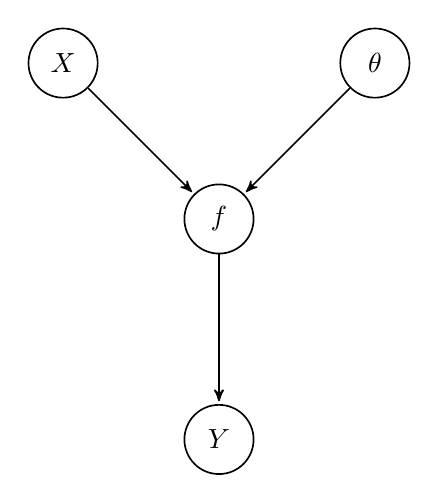
\begin{tikzpicture}[->,>=stealth',shorten >=1pt,auto,node distance=2.8cm,
                    semithick]
  

  \node[state] (Y)                    {$Y$};
  \node[state]         (f) [above of=Y] {$f$};
  \node[state]         (O) [above right of=f] {$\theta$};
  \node[state]         (X) [above left of=f] {$X$};

  \path (O) edge              node {} (f)
        (X) edge              node {} (f)
        (f) edge              node {} (Y);
\end{tikzpicture}
\caption{Graphical model for non-parametric representation learning}
\label{graphical}
\end{figure}

\subsection{Practical}
\subsubsection{Linear Representation Learning}
\fbox{
  \parbox{\textwidth}{
\textbf{Question 21: }\textit{
Plot the representation that you have learned. Explain why it looks the way it
does. Was this the result that you expected? Hint: Plot X as a two-dimensional representation.
}}}
\smallskip\\
We recover the type-II maximum likelihood estimate for the linear mapping W: 
\begin{equation*}
\hat{W} = argmin_W \; \mathcal{L}(W)
\end{equation*}
We can then write:
\begin{align*}
Y &= X'\hat{W}^T\\
Y\hat{W} &= X'\hat{W}^T\hat{W}\\
X' &= Y\hat{W}(\hat{W}^T\hat{W})^{-1}
\end{align*}
When comparing the actual $X'$ (figure \ref{actual}) and the representation of $X'$ that we have learned (figure \ref{recovered}), we can see that while their shapes are similar, one is a rotated version of the other. Since the marginal likelihood that we maximize has the following form:
\begin{equation*}
P(Y|W) = \prod\limits_{i=1}^{N}\mathcal{N}(y_i| 0 , WW^T + \sigma^2I)
\end{equation*}
For all $\hat{W}= WR$ :
\begin{equation*}
\begin{split}
P(Y|\hat{W}) &= \prod\limits_{i=1}^{N}\mathcal{N}(y_i| 0 , WRR^TW^T + \sigma^2I)\\
&=\prod\limits_{i=1}^{N}\mathcal{N}(y_i| 0 , WW^T + \sigma^2I)
\end{split}
\end{equation*}
The likelihood is invariant to a rotation of $W$. Therefore, all the linear mappings $\hat{W}= WR$ are solutions, which explains the difference in the direction of rotation between the actual and the learned $X'$.

\begin{figure}[h]
\centering
\includegraphics[scale =0.75]{awesome} 
\caption{Learned representation of $X'$}
\label{recovered}
\end{figure}

\begin{figure}[h]
\centering
\includegraphics[scale =0.75]{actualx}
\caption{Actual $X'= [X\odot sin(X),X \odot cos(X)]$ where $X = [0...4\pi]^T$ }
\label{actual}
\end{figure}
\clearpage




\section{The Evidence $p(Y)$}
\subsection{Theory}
\subsubsection{Data}
\subsubsection{Models}
\fbox{
  \parbox{\textwidth}{
\textbf{Question 22: }\textit{
Why is this the simplest model, and what does it actually imply? Discuss its
implications, why is this a bad model and why is it a good model.
}}}
\smallskip
\\$M_0$ is the simplest model because it has no free parameters: it assigns all datasets an equal probability of $1\over152$. It has the advantage of having the largest evidence over all the range of possible data-sets, but it since it uses no information about the actual data-set, it is unable to assign much probability mass to simple data-sets.\\\\
\fbox{
  \parbox{\textwidth}{
\textbf{Question 23: }\textit{
Explain how each separate model works? In what way is this model more or
less flexible compared to M0? How does this model spread its probability mass over D?
}}}
\smallskip
\\Given $\theta_i$, each model gives see how well a point $x^i$ is separable by the decision boundary $\theta_1^1x^i=0$ where one side of which has $y=1$ and the other one has $y=-1$. If $y^i$ corresponds to the right position of the point with respect to the boundary then, $p \geq 0.5$.\\
$M_1$ is similar to standard logistic regression but it only takes into account the first dimension of $x$. $M_1$ will give a higher probability to data-sets with sharp linear decision boundaries that are a function of $x_1$, and not $x_2$: it means that it is more adaptable to this category of data-sets. $M_1$ concentrates its probability mass around this limited number of data-sets, while $M_0$ predicts that the data will be drawn from a large number of data-sets, thus spreading its unit probability mass over a wider range. 
\smallskip
\\\\
\fbox{
  \parbox{\textwidth}{
\textbf{Question 24: }\textit{
How have the choices we made above restricted the distribution of the model?
What data sets are each model suited to model? What does this actually imply in terms of
uncertainty? In what way are the different models more 
flexible and in what way are they more
restrictive? Discuss and compare the models to each other?
}}}
\smallskip
\\
$M_2$ will give a higher probability to data-sets with decision boundaries crossing the origin, while $M_3$ with the bias term $\theta_0$ allows decision boundaries to be offset from the origin. $M_3$, is the most complex model of the four in the sense that it has the most
parameters and can realize the other models by setting
some of its parameters to zero. This means that we expect
it to spread the important part of its unit probability mass over
a wider range of data sets than the other models. However, this flexibility means that when the observed data can be explained by a simpler model, $M_3$ will be penalized since it has spent its probability mass elsewhere.
\smallskip
\\\\
\fbox{
  \parbox{\textwidth}{
\textbf{Question 25: }\textit{
Explain the process of marginalisation. Discuss its implications.
}}}
\smallskip
\\Being Bayesians, we express our believes about the parameter $\theta$ by specifying a prior over $\theta$. We then find the evidence of the model $p(D|M_i)$ by averaging $p(D|M_i, \theta)$ over all possible values of the parameter $\theta$, using the prior $p(\theta)$ as a weight for each of these values: we average according to our beliefs. The evidence can also be viewed as the probability
of generating the data set D from a model whose parameters are sampled randomly from the prior.
\smallskip
\\\\
\fbox{
  \parbox{\textwidth}{
\textbf{Question 26: }\textit{
What does this choice of prior imply? How does the choice of the parameters of
the prior $\mu$ and $\Sigma$ affect the model?
}}}
\smallskip
\\The prior on the parameters $p(\theta | M_i) = \mathcal{N}(0, 10^3I)$ implies :
\begin{itemize}
\item The components (dimensions) of the vector $\theta$ are independent.
\item The standard deviation is $10^{3\over2}$: it means that we favour settings of the parameter $\theta$ which correspond in x space to sharp linear boundaries. Therefore we assume data-sets with sharp linear boundaries to be typical. 
\end{itemize}
\hfill \\
\fbox{
  \parbox{\textwidth}{
\textbf{Question 27: }\textit{
For each model sum the evidence for the whole of D what numbers do you get?
Explain these numbers for all the models and relate them to each other.
}}}
\smallskip
\\By construction of $p(D|M,\theta)$ for all possible data-sets, the evidence sums to one (for each model). 
\smallskip
\\\\
\fbox{
  \parbox{\textwidth}{
\textbf{Question 28: }\textit{
Plot the evidence over the whole data set for each model. The x-axis index the
different instances in D and each models evidence is on the y-axis. How do you interpret this,
relate this to the parametrisation of each model.
}}}
\smallskip
\\The evidence plot in figure \ref{evidencePlot} confirms that $M_0$ has the largest evidence over all the range of possible data-sets. \\
We can also see that the models $M_1$, $M_2$ and $M_3$ are nested in the sense that a model with a higher number of parameters could represent another by setting some of its parameters to 0. Therefore, we can see that $M_3$ assigns probability mass to all the data-sets predicted by $M_1$ and $M_2$, but it is outperformed by them in some ranges that would correspond to data-sets with simple decision boundaries.\\
The range where the evidence given by $M_2$ and $M_3$ is maximal and similar ($D \leq 10$) would correspond to data-sets with vertical or almost vertical boundaries that are well-modeled by both, with an advantage for $M_1$ that is simpler and therefore has more probability mass to assign to them. When the evidence given by $M_2$ is maximal, the data-sets would still have simple boundaries(linear and crossing the origin), but with orientations that cannot be captured by $M_1$ because it is only a function of $x_1$.\\
When ($D \geq 25$), we are in the range of data-sets with more complex boundaries that can only be modeled by $M_3$ because it's the only model with a bias term.
\smallskip\\\\
\begin{figure}[h]
\begin{subfigure}{0.5\textwidth}
\includegraphics[scale=0.43]{all}
\caption{Plot over all possible data-sets}
\label{all}
\end{subfigure}
\begin{subfigure}{0.5\textwidth}
\includegraphics[scale=0.43]{zoom}
\caption{zoom over a subset of possible data-sets}
\label{zoom1}
\end{subfigure}
\caption{Plots of evidence for possible data-sets $\mathcal{D}$ for the models}
\label{evidencePlot}
\end{figure}
\fbox{
  \parbox{\textwidth}{
\textbf{Question 29: }\textit{Find using np.argmax and np.argmin which part of the D that is given most
and least probability mass by each model. Plot the data-sets which are given the highest and
lowest evidence for each model. Discuss these results, does it make sense?
}}}
\\
\begin{description}
\item[Model 0]\hfill \\
All data-sets have the same probability under $M_0$
\item[Model 1] \hfill \\
$M_1$ captures decision boundaries that are functions of $x_1$ and not $x_2$. The data-set in table \ref{max1} has a simple boundary that is a function of x1 (since the different point has $x_1 = 0$, which explains why $M_1$ would give it a high probability.\\
The data-set in table \ref{min1} has a complex boundary (the points are non-linearly separable), which explains why it has a low probability.
\begin{table}[h]
    \caption{Model 1}
    \begin{minipage}{.5\linewidth}
      \caption{Most probable data-set}
      \label{max1}
      \centering
        \begin{tabular}{c|c|c}
          O & O & X \\
          \hline
          O & O & X \\
          \hline
          O & X & X
        \end{tabular}
    \end{minipage}%
    \begin{minipage}{.5\linewidth}
      \centering
        \caption{Least probable data-set}
        \label{min1}
        \begin{tabular}{c|c|c}
          O & X & O \\
          \hline
          X & X & O \\
          \hline
          O & X & X
        \end{tabular}
    \end{minipage} 
\end{table}
\item[Model 2] \hfill \\
$M_2$ is standard logistic regression without the bias term $\theta_0$, so it models decision boundaries that cross the origin. It makes sens that the data-set in table \ref{max2} has a high probability under $M_2$. \\
Similarly to $M_1$, the data-set with the lowest probability for $M_2$ (table \ref{min2}) has a complex non-linear boundary.

\begin{table}[h]
    \caption{Model 2}
    \begin{minipage}{.5\linewidth}
      \caption{Most probable data-set}
      \label{max2}
      \centering
        \begin{tabular}{c|c|c}
          O & O & O \\
          \hline
          X & O & O \\
          \hline
          X & X & X
        \end{tabular}
    \end{minipage}%
    \begin{minipage}{.5\linewidth}
      \centering
        \caption{Least probable data-set}
        \label{min2}
        \begin{tabular}{c|c|c}
          X & O & O \\
          \hline
          X & O & X \\
          \hline
          O & O & O
        \end{tabular}
    \end{minipage} 
\end{table}
\item[Model 3] \hfill \\
$M_3$ has a bias term that allows decision boundaries to be offset from the origin; the prior on
the parameter $\theta_3$, has width $10^{3\over2}$, which favors sharp linear boundaries (possibly large intercepts), both of which are consistent with the data-set in table \ref{max3}.
\begin{table}[h]
    \caption{Model 3}
    \begin{minipage}{.5\linewidth}
      \caption{Most probable data-set}
      \label{max3}
      \centering
        \begin{tabular}{c|c|c}
          X & X & X \\
          \hline
          X & X & X \\
          \hline
          X & X & X
        \end{tabular}
    \end{minipage}%
    \begin{minipage}{.5\linewidth}
      \centering
        \caption{Least probable data-set}
        \label{min3}
        \begin{tabular}{c|c|c}
          O & X & O \\
          \hline
          O & O & X \\
          \hline
          X & O & O
        \end{tabular}
    \end{minipage} 
\end{table}

\end{description}
\smallskip
\fbox{
  \parbox{\textwidth}{
\textbf{Question 30: }\textit{
What is the effect of the prior $p(\theta)$.
\begin{itemize}
\item What happens if we change its parameters?
\item What happens if we use a non-diagonal covariance matrix for the prior?
\item Alter the prior to have a non-zero mean, such that $\mu = [5, 5]^T$?
\item Redo evidence plot for these and explain the changes compared to using zero-mean.
\end{itemize}
}}}
\smallskip
\begin{figure}[ht]
\begin{subfigure}{0.5\textwidth}
\includegraphics[scale=0.43]{mean2}
\caption{Plot over all possible data-sets}
\label{nonzero}
\end{subfigure}
\begin{subfigure}{0.5\textwidth}
\includegraphics[scale=0.43]{mean2zoom}
\caption{zoom over a subset of possible data-sets}
\label{nonzerozoom}
\end{subfigure}
\caption{Evidence for possible data-sets $\mathcal{D}$ with $p(\theta|M_i) = \mathcal{N}(\mu,\Sigma)$, where $\mu = [5,5]^T$}
\label{evidencePlotmean}
\end{figure}
\begin{itemize}
\item We saw from our experiments that a prior with a large variance favored sharp decision boundaries, which happens for large settings of the parameters $\theta$. If we had chosen a prior with a smaller variance, then the models would have given a more uniform evidence, similarly to $M_0$.
\item With a non-diagonal covariance matrix for the prior, the parameters $\theta_n$ (components of the vector $\theta$) become dependent. Certain data-sets would become more or less probable depending on the value and sign of the correlation between the parameters. For example in $M_3$, if $\theta_1$ and $\theta_2$ are positively correlated with each other and negatively correlated with $\theta_0$, the data-sets with a slope and and intercept that have different signs will be assigned a higher probability.
\item The evidence plot for a prior with a non-zero mean (figure \ref{evidencePlotmean}) show evidence distributions that are more peaked around certain data-sets for all models. We can therefore conclude that a non-zero mean assigns a larger probability mass to specific data-sets, for which the boundaries correspond to parameter values around this mean.
\end{itemize}
\end{document}
